\subsection{Simulation 2}
\label{sec:sim2}

This second numerical exercise focuses on the asymptotic behavior of the LCC estimate. The focal point is Theorem 8 in Section \ref{sec:lcc-asymp}, which states that if the model is correctly specified and the pilot model is consistent and independent of the data, the asymptotic variance of the local case-control estimate will be precisely twice the asymptotic variance of the logistic regression estimate on the full sample. As stated before, the simulation study uses a data-dependent pilot since, according to the authors, an independent one would require, for example, fitting the model in data from an earlier period.\\

Consider the simulation setup in \ref{sec:sim_general}, this time with $k=30$ and full population sizes of $N=\{10^5, 10^6\}$ that aim to approximate the asymptotic limit behavior. For this part of the analysis, there are no fixed subsample sizes $N_s$ neither for the pilot nor the LCC algorithm. Rather, the pilot estimates $\Tilde{\theta}$ are taken from an initial pass on the whole data set, and the LCC subsample should be roughly $n\Bar{a}(\Tilde{\theta})$. The results are shown in Table \ref{tab:sim2}. Both methods are asymptotically unbiased, and so it is observed in the table results, where the squared bias of both logistic regression and LCC are approaching zero.\\

As for the variance's relation between LCC and the logit model, the results show that for $N=10^5$, the LCC's variance is approximately $2.85$ times the variance of the logistic regression. Letting the full population size increase to $N=10^6$ reduces this factor to  $2.66$. There are two possible reasons why the LCC's variance might not be exactly twice as of the logit for this exercise. First, since it is an asymptotic result, much larger population size might be needed to approximate the asymptotic behavior of the LCC estimate. And secondly, the theoretical results assume a data-independent pilot, which in this case, does not hold. A data-dependent pilot could be inflating the variance of the LCC in finite samples.

\begin{table}[ht]
\centering
\begin{tabular}{lccccccccc}
    \toprule
    & \multicolumn{4}{c}{$N=10^5$} & \multicolumn{4}{c}{$N=10^6$}\\
    \cmidrule(lr){2-5}\cmidrule(lr){6-9}
    \multicolumn{1}{c}{} & \multicolumn{1}{c}{$\Bar{N_s}$} &\multicolumn{1}{c}{$\widehat{bias}^2$} & \multicolumn{1}{c}{$\widehat{var}$} & \multicolumn{1}{c}{$\Bar{a}(\Tilde{\theta})$} & \multicolumn{1}{c}{$\Bar{N_s}$} &\multicolumn{1}{c}{$\widehat{bias}^2$} & \multicolumn{1}{c}{$\widehat{var}$} & \multicolumn{1}{c}{$\Bar{a}(\Tilde{\theta})$}\\
    \midrule
    Logit & $10^5$ & 0.0012 & 0.0279 & -
    & $10^6$ & $8.47 \times 10^{-6}$ & 0.0027 & -\\
    LCC & 2140 & 0.0003 & 0.0796 &  0.0214 
    & 21394 & $3.71\times 10^{-6}$ & 0.0072 & 0.0214\\
    \bottomrule
\end{tabular}
\caption[Simulation 2 - Approximation of asymptotic behavior of LCC against logit]{Simulation 2 - Approximation of asymptotic behavior of LCC against logit (results for 1,000 runs).}
\label{tab:sim2}
\end{table}

\begin{figure}[ht]
    \centering
    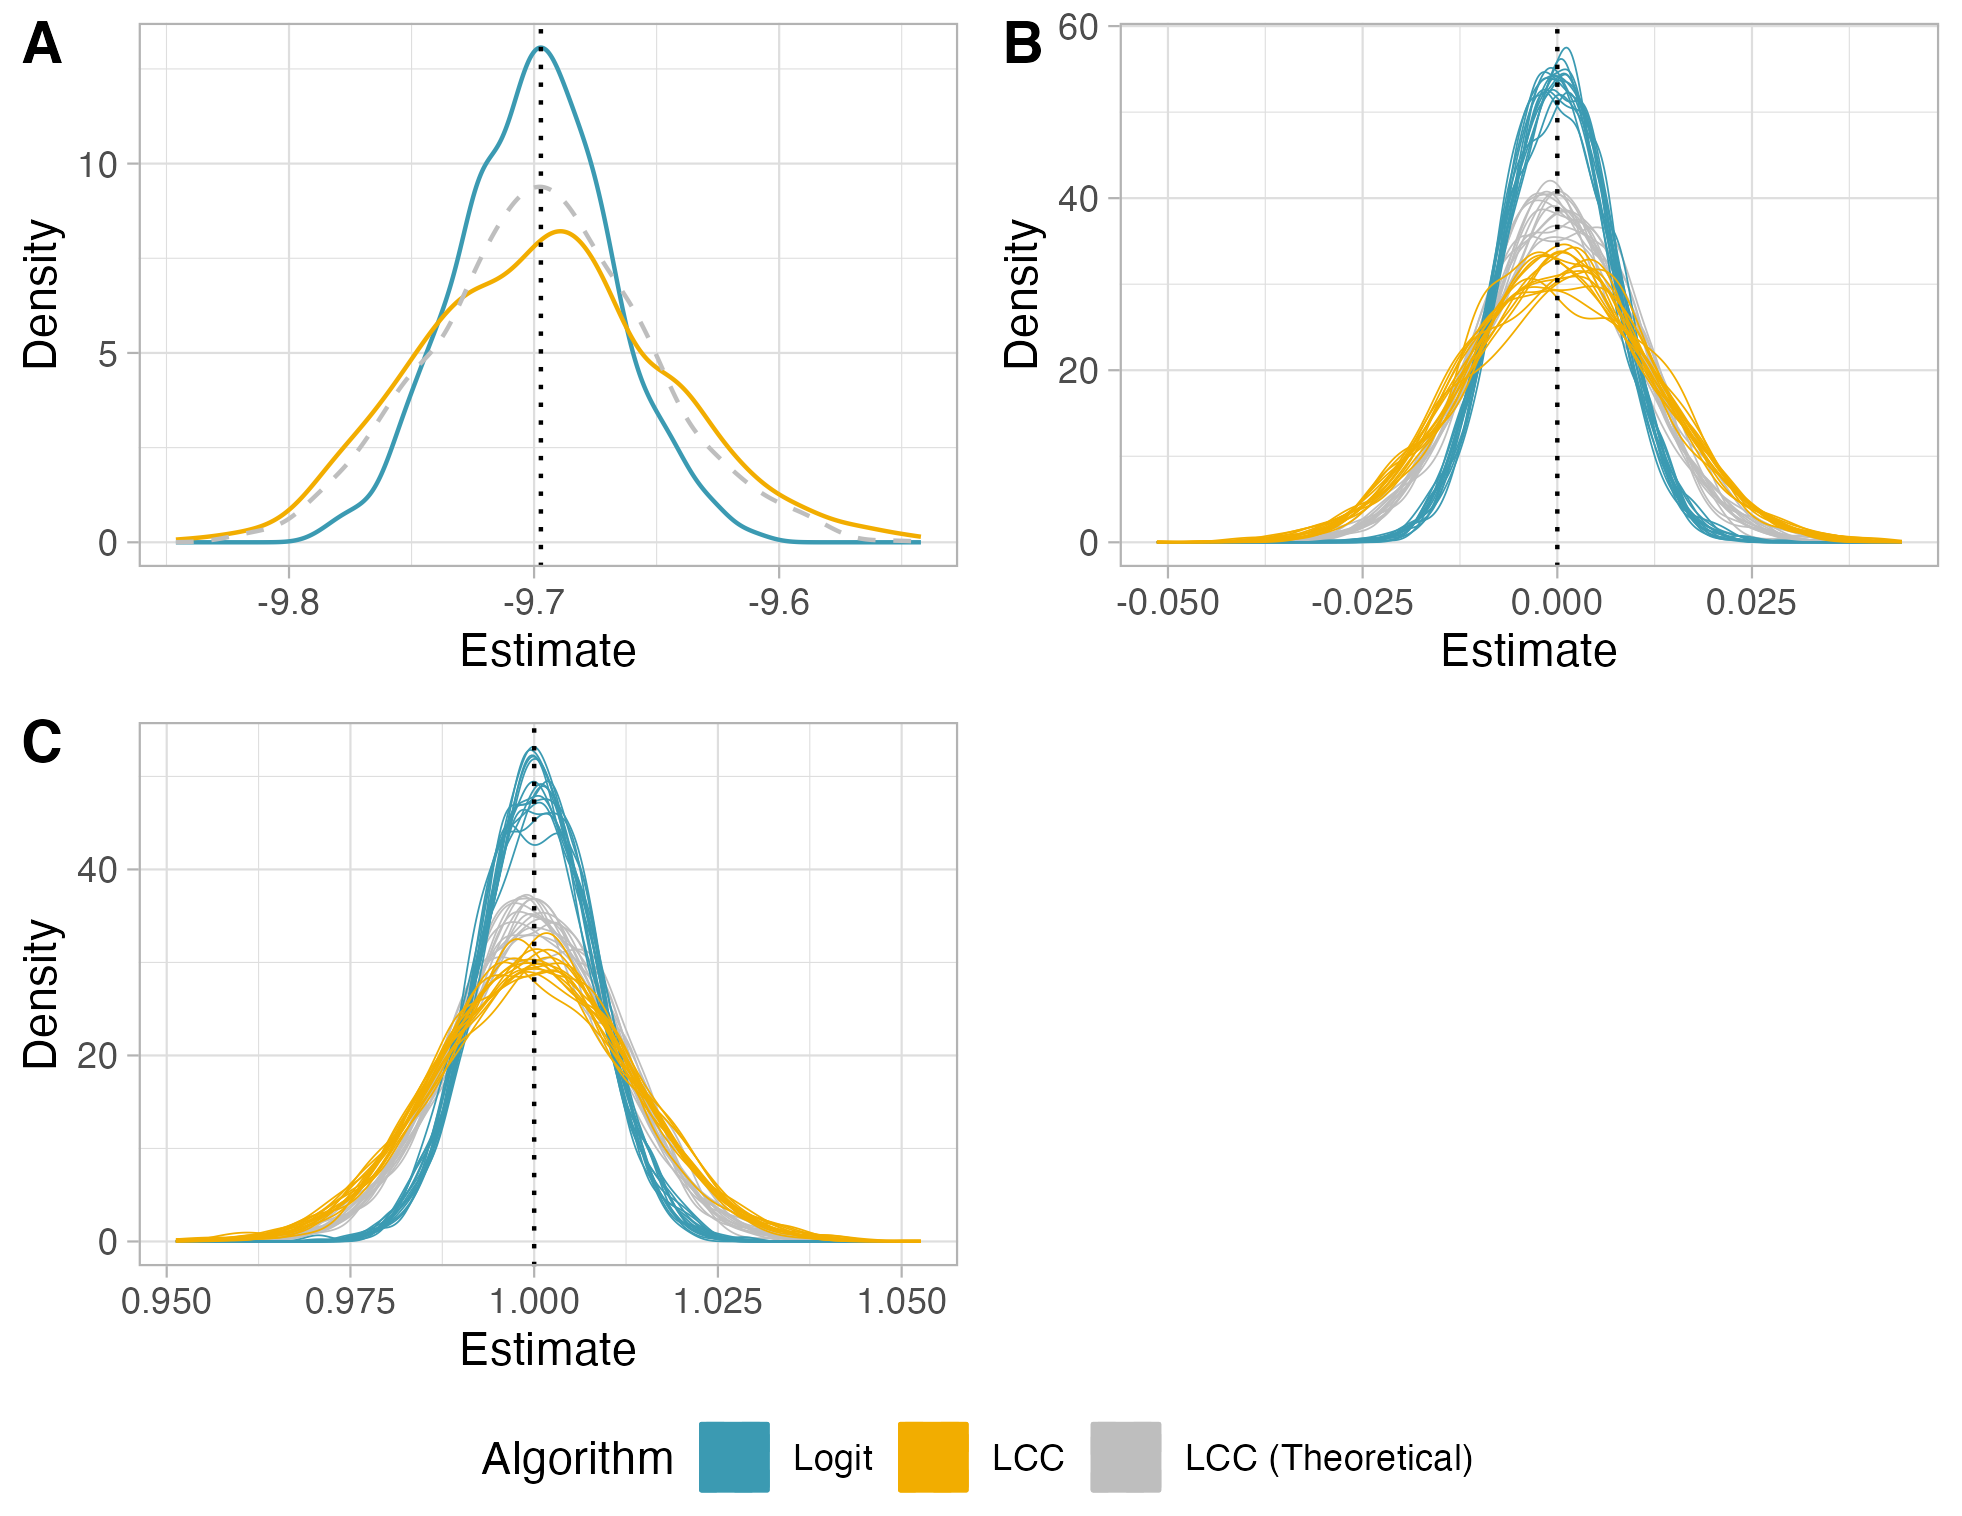
\includegraphics[width=\textwidth]{2_Figures/all_densities.png}
    \caption[Simulation 2 - Distribution of Monte Carlo realizations $\hat{\theta}_{logit}$, $\hat{\theta}_{LCC}$ and theoretical $\hat{\theta}_{LCC}$]{Simulation 2 - Approximation of $\hat{\theta}$ asymptotic distributions across methods for $N=10^6$, where the grey line corresponds to the theoretical distribution of the LCC estimate (results from $1,000$ runs). \textbf{Panel A}: True $\alpha=-9.7$ 
    \textbf{Panel B}: True $\beta=0$, namely $\beta_1, \dots, \beta_{\frac{k}{2}}=0$. 
    \textbf{Panel C}: True $\beta=1$, namely $\beta_{\frac{k}{2}+1}, \dots, \beta_k=1$.}
    \label{fig:all_densities}
\end{figure}

Although the simulation findings do not match the theoretical predictions exactly, they are still very close. Figure \ref{fig:all_densities} shows the different distributions of the Monte Carlo simulations, distinguishing between $\hat{\alpha}$'s distribution, one $\hat{\beta}$ distribution for $\beta_1, \dots, \beta_{\frac{k}{2}}=0$ and one $\hat{\beta}$ distribution for $\beta_{\frac{k}{2}+1}, \dots, \beta_k=1$. The grey distribution represents the theoretical distribution for each set of estimates. It is shown that despite not fitting it perfectly, the LCC distribution closely follows the theoretical one for all sets of estimates. It is worth noting that $\Bar{a}(\Tilde{\theta})=0.0214$, which means that despite only using approximately $2\%$ of the complete sample, LCC's variance is still no larger than $3$ times the logit variance for large samples.


% The results show that, for this specific setup of the DGP, that is, high conditional imbalance and large population size, LCC outperforms logistic regression in terms of $\widehat{bias^2}$ for both $N= 10^5$ and $N=10^6$. On the other hand, the theory says that the asymptotic variance of the LCC algorithm should be exactly twice the variance of logistic regression on the full sample. In this case, the results come close to what the theory predicts, with the variance of the LCC being roughly 2.8 times the variance of logistic regression for $N=10^5$ and 2.7 for the case when the population size is $N=10^6$. The more $N \to \infty$, the closer the results will get to the theory described by \cite{hastie2014}.\\
